


%%%%%%%%%%%%%%%%%%%%%%%%%%%%%%%%%%%%%%%%%%%%%%%%%%%%%%%%%%%%%%%%%%%%%%%%%%%%%%
\section{RPC on hydrogen}

The energy spectrum of photons produced in the process of RPC on hydrogen \cite{RPC_1972_Bistirlich_PhysRevC.5.1867} is shown if Figure~\ref{figure:1971_bistirlich_fig_02_h2}.
The peak at 129.4 MeV corresponds to photons produced in the $\pi^- p \to n \gamma$ reaction,
  The low energy part of the spectrum is populated by the photons from decays of $\pi^0$ produced
  in the $\pi^- p \to n \pi^0$ reaction. The photons have been reconstructed in a $\gamma \to e^+e^-$
  mode with the electron and positron momenta reconstructed in the magnetic spectrometer.

The 129.4 MeV $\pi^{-} p \to n \gamma$ peak is also clearly seen on hydrogen-containing compounds.
  Figure~\ref{figure:1971_bistirlich_fig_09_ch2}, also taken from \cite{RPC_1972_Bistirlich_PhysRevC.5.1867},
  shows the photon energy spectrum from RPC on a $CH_2$ target.
  There is a clear separation between the contributions of $H$ and $C_{12}$,
  and the part of the spectrum in between 90 and 120 MeV is dominated by the photons from RPC on $C_{12}$

To produce a 129.4 MeV photon, (i) a negative pion stopped on a $\rm{CH_2}$  degrader must be captured on a hydrogen rather
than carbon nucleus, and (ii) the capture must be followed by a $\pi^{-} p \to n \gamma$ reaction.


\begin{figure}[H]
 \begin{minipage}{.5\textwidth}
  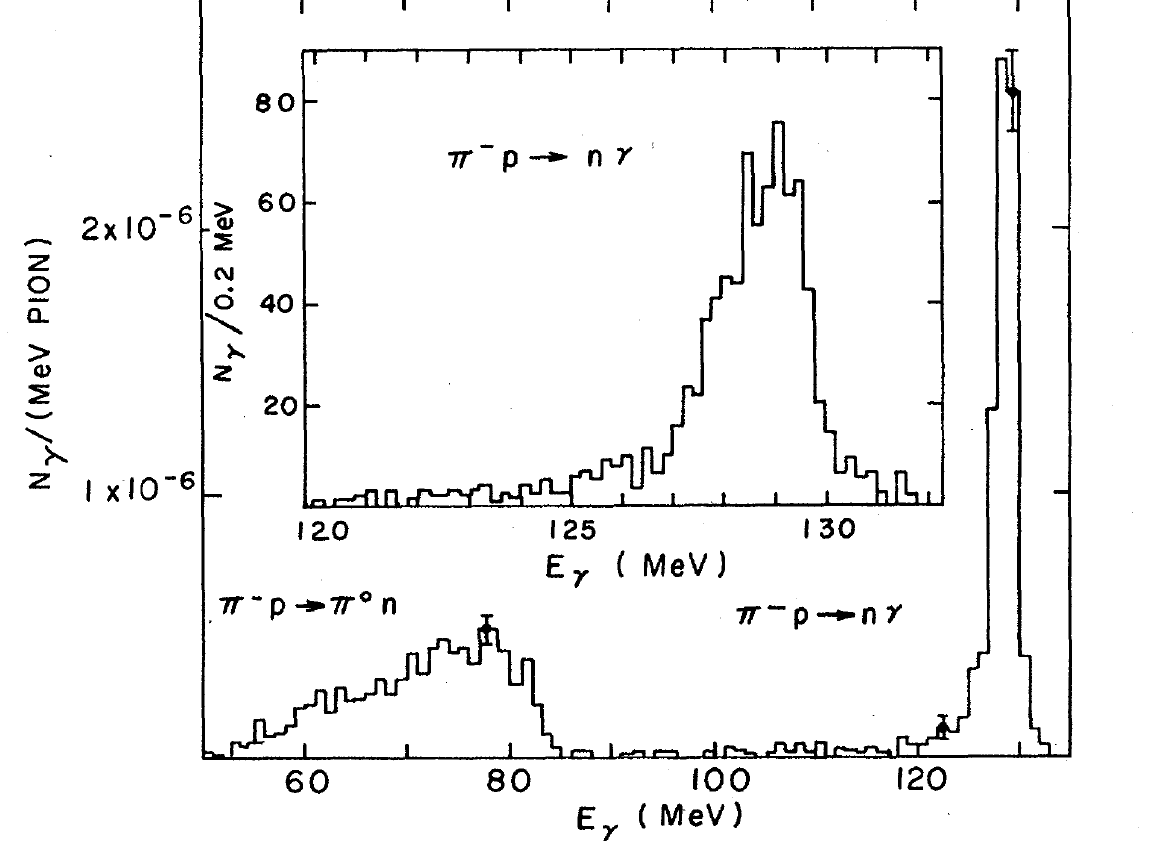
\includegraphics[width=0.9\textwidth]{png/1971_bistirlich_fig_02_h2}
  \captionsetup{width=.8\linewidth}
  \caption[width=0.9\textwidth]{
      \label{figure:1971_bistirlich_fig_02_h2}
    Photon energy spectrum from negative pion capture on hydrogen \cite{RPC_1972_Bistirlich_PhysRevC.5.1867}.
    }
 \end{minipage}
 \begin{minipage}{.5\textwidth}
  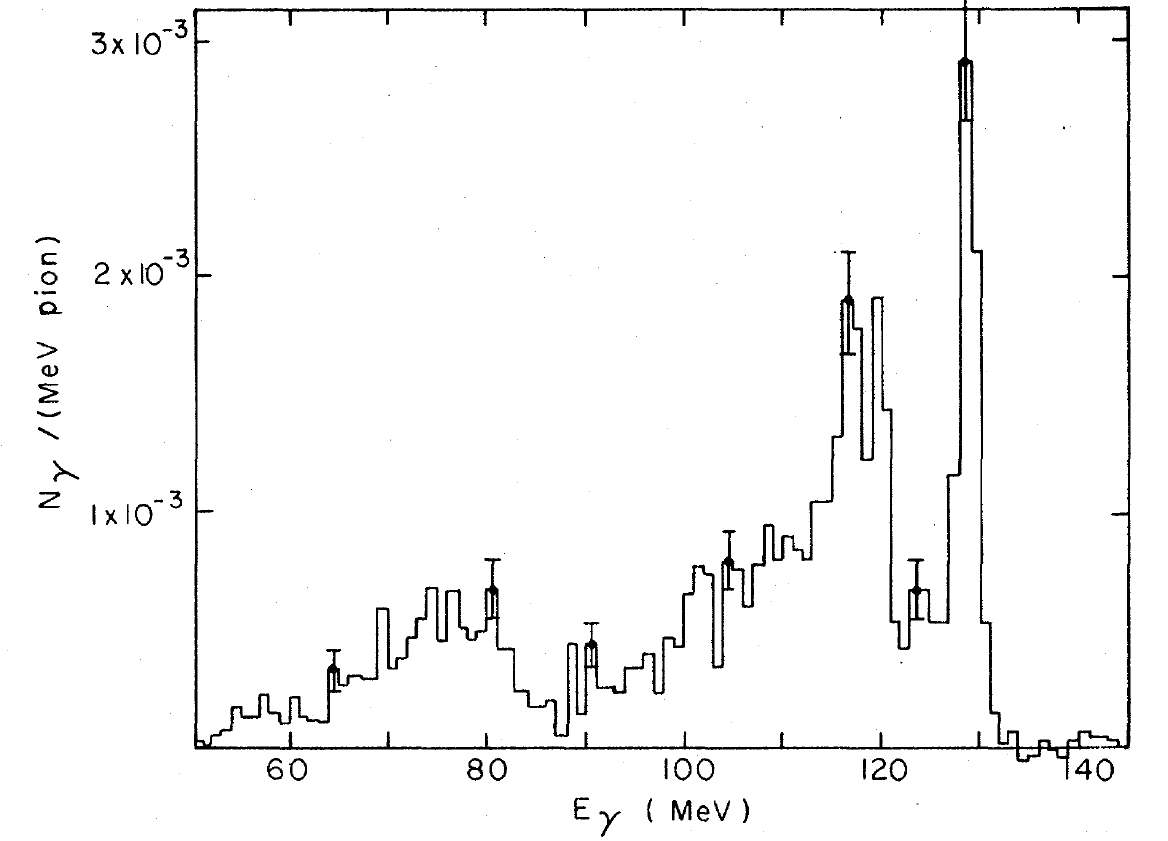
\includegraphics[width=0.9\textwidth]{png/1971_bistirlich_fig_09_ch2}
  \captionsetup{width=.8\linewidth}
  \caption[width=0.9\textwidth]{
  \label{figure:1971_bistirlich_fig_09_ch2}
    Photon energy spectrum from negative pion capture on $\rm{CH_2}$ \cite{RPC_1972_Bistirlich_PhysRevC.5.1867}.
   }
 \end{minipage}
\end{figure}

The probability of pion capture on the hydrogen component of the $\rm{CH_2}$ compound is
$\newline \rm{ W_H = (12.9 \pm 1.8) \times 10^{-3 }}$
 as used in Ref.~\cite{RPC_1991_Harston_PhysRevA.44.103}
 , an average of previous measurements. 
 This accounts for both hydrogen atoms in the $\rm{CH_2}$ molecule, and is larger than but consistent with the
 corresponding measurement (expressed as percent) in Ref.~\cite{RPC_1972_Bistirlich_PhysRevC.5.1867}.
 Negative pions captured on hydrogen have a $ (41.4 \pm 3.2) \% $
 probability of interacting via $\pi^{-} p \to n \gamma$ and producing a photon at 129.4 MeV
 \cite{RPC_1972_Bistirlich_PhysRevC.5.1867}.
 The remaining pions captured on hydrogen produce two photons via the charge exchange reaction
 $ \pi^{-} p \to n \pi^0 $ with $\pi^0  \to \gamma \gamma $,
 which results in the lower energy peak of the hydrogen spectrum. 

Together these factors yield a probability of around $ 5 \times 10^{-3} $
for obtaining 129.4 MeV RPC photons from pion capture on $\rm{CH_2}$.



%%% Local Variables:
%%% mode: latex
%%% TeX-master: t
%%% End:
